The C preprocessor is a program that processes the source program before it is passed to the compiler. There are several steps involved from the stage of writing a C program to the stage of getting it executed. \figref{CCodingSteps} shows these different steps along with the files created during each stage. The input and output to each of these processors is shown in \figref{CCodingStepsIO}.

\begin{figure}[H]
    \begin{center}
        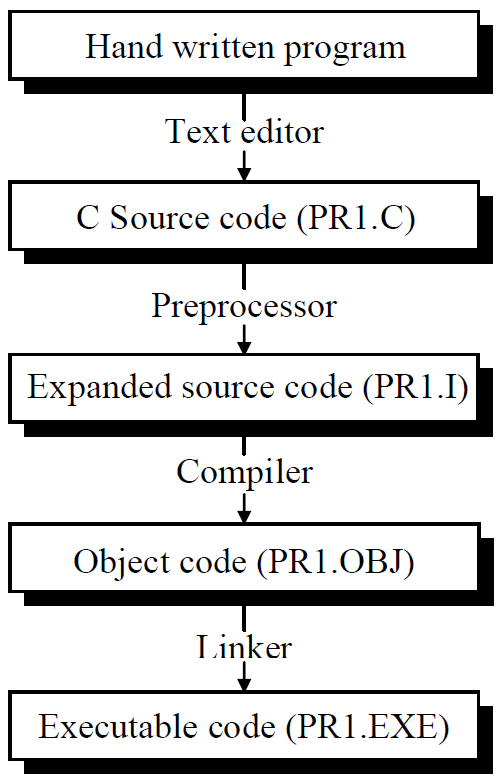
\includegraphics[width=0.45\textwidth]{images/CCodingSteps.PNG}
        \caption{Different stages of a C program}
        \label{CCodingSteps}
    \end{center}
\end{figure}


\begin{figure}[H]
    \begin{center}
        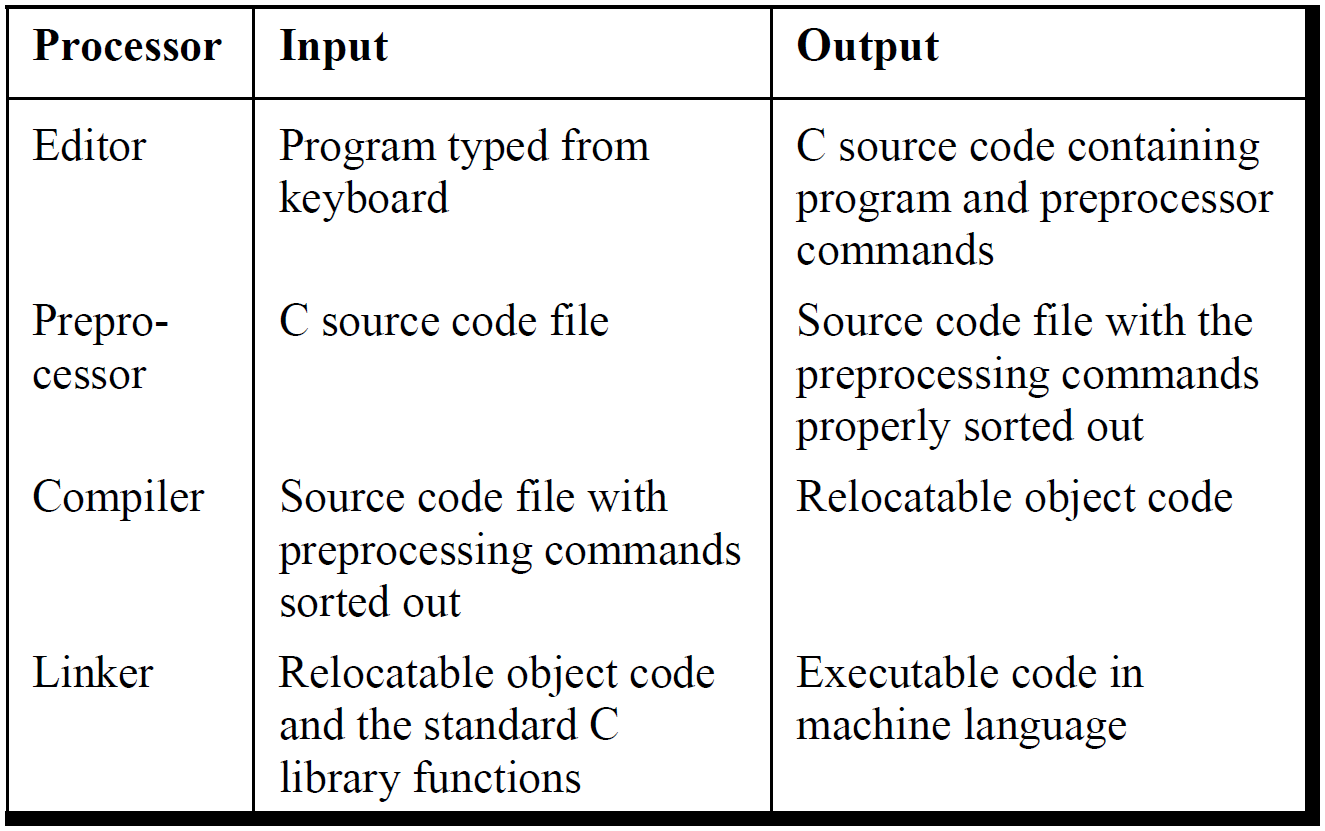
\includegraphics[width=0.8\textwidth]{images/CCodingStepsIO.PNG}
        \caption{Input and Output to each stage of a C program}
        \label{CCodingStepsIO}
    \end{center}
\end{figure}

Note that if the source code is stored in a file PR1.C then the expanded source code gets stored in a file PR1.I. When this expanded source code is compiled, the object code gets stored in PR1.OBJ. When this object code is linked with the object code of library functions the resultant executable code gets stored in PR1.EXE.

\par The preprocessor offers several features called preprocessor directives. Each of these preprocessor directives begin with a \# symbol. The directives can be placed anywhere in a program but are most often placed at the beginning of a program, before the first function definition. Preprocessor replaces preprocessor directives (starting with \#) with actual content before compilation. 

There are 4 main types of preprocessor directives: 
\begin{enumerate}
    \item Macro expansion
    \item File Inclusion
    \item Conditional Compilation
    \item Miscellaneous directives
\end{enumerate} 

\subsection{Macro expansion}

Macros are a piece of code in a program which is given some name. Whenever this name is encountered by the compiler the compiler replaces the name with the actual piece of code. The '\#define' directive is used to define a macro. 

\begin{itemize}
    \item Note: There is no semi-colon(';') at the end of macro definition. Macro definitions do not need a semi-colon to end.
    \item In C programming it is customary to use capital letters for macro template.
    \item Macros can have arguments.
    \item In a macro call the preprocessor replaces the macro template with its macro expansion, unlike in a function call the control is passed to a function along with certain arguments, some calculations are performed in the function and a useful value is returned back from the function.
    \item Usually macros make the program run faster but increase the program size, whereas functions make the program smaller and compact.
\end{itemize}


\subsection{File Inclusion}
File Inclusion preprocessor directive tells the compiler to include a file in the source code program. There are two ways of writing \#include statement:

\begin{lstlisting}[style=CStyle]
    #include "filename" // This command looks for the file in the current directory as well as the specified list of directories as mentioned in the include search path that might have been set up.
    
    #include <filename> // This command would look for the file in the specified list of directories only.
\end{lstlisting}

There are two types of files which can be included by the user in the program: 
\begin{enumerate}
    \item Header File or Standard files: These files contains definition of pre-defined functions like printf(), scanf() etc. These files must be included for working with these functions. Different function are declared in different header files. \eg standard I/O functions are in 'iostream' file whereas functions which perform string operations are in 'string' file.
    \item user defined files: When a program becomes very large, it is good practice to divide it into smaller files and include whenever needed. These types of files are user defined files. 
\end{enumerate}

\subsection{Conditional Compilation}
Conditional Compilation directives are type of directives which helps to compile a specific portion of the program or to skip compilation of some specific part of the program based on some conditions. This can be done with the help of two preprocessing commands 'ifdef' and 'endif'. 

\begin{lstlisting}[style=CStyle]
    #ifdef macroname
        statement 1 ;
        statement 2 ;
        statement 3 ;
    #endif
\end{lstlisting}

\par If the macro with name as 'macroname' is defined then the block of statements will execute normally but if it is not defined, the compiler will simply skip this block of statements. Usecases of Conditional Compilation directives are:

\begin{enumerate}
    \item To comment out or include part(s) of a code with a single definition of a macro.
    \item A more sophisticated use of \#ifdef has to do with making the programs portable, i.e. to make them work on two totally different computers.
    \item \#ifndef is used to avoid multiple definitions , declaration, and or inclusions.
\end{enumerate}

\subsubsection{\#if and \#elif Directives}
The \#if directive can be used to test whether an expression evaluates to a nonzero value or not. If the result of the expression is nonzero, then subsequent lines upto a \#else, \#elif or \#endif are compiled, otherwise they are skipped.



\subsection{Miscellaneous directives}
Apart from the above directives there are two more directives which are not commonly used. These are: 

\subsubsection{\#undef Directive} 
The \#undef directive is used to undefine an existing macro. Using this statement will undefine the existing macro. After this statement every \#ifdef statement will evaluate to false. 

\subsubsection{\#pragma Directive}
This directive is a special purpose directive and is used to turn on or off some features. This type of directives are compiler-specific, \ie they vary from compiler to compiler. Some of the \#pragma directives are discussed below: 

\paragraph{\#pragma startup and \#pragma exit}
These directives helps us to specify the functions that are needed to run before program startup (before the control passes to main()) and just before program exit (just before the control returns from main()). 

\paragraph{\#pragma warn Directive}
This directive is used to hide the warning message which are displayed during compilation. 

\begin{itemize}
    \item \#pragma warn -rvl: This directive hides those warning which are raised when a function which is supposed to return a value does not returns a value.
    \item \#pragma warn -par: This directive hides those warning which are raised when a function does not uses the parameters passed to it.
    \item \#pragma warn -rch: This directive hides those warning which are raised when a code is unreachable. \eg any code written after the return statement in a function is unreachable.
\end{itemize}



\iffalse

As the name suggests Preprocessors are programs that process our source code before compilation. There are a number of steps involved between writing a program and executing a program in C / C++. 


\begin{figure}[H]
    \begin{center}
        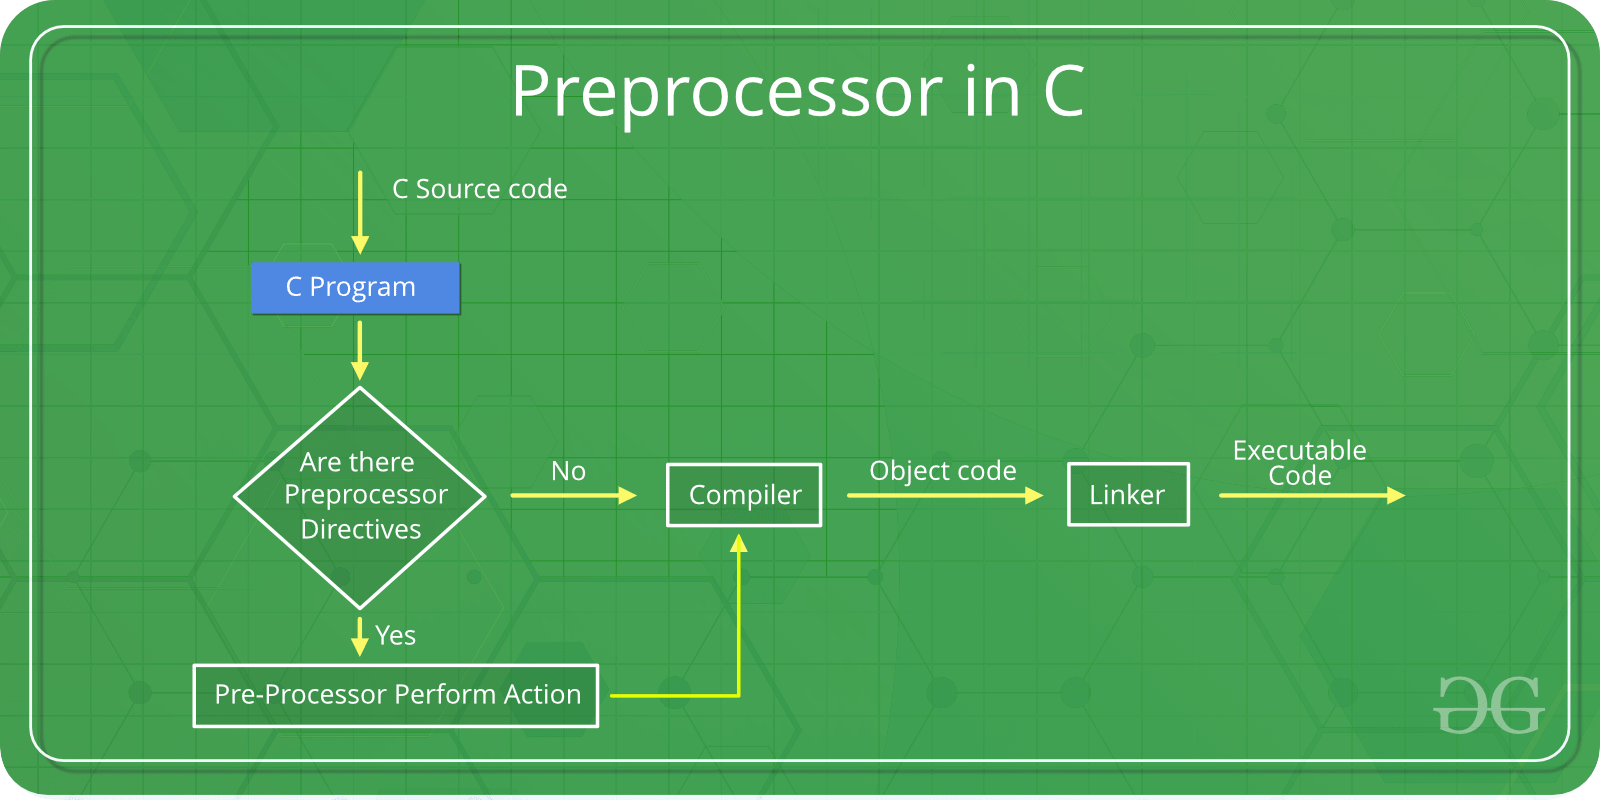
\includegraphics[width=0.6\textwidth]{images/Cpreprocessor.png}
        \caption{Preprocessor in C}
        \label{Cpreprocessor}
    \end{center}
\end{figure}

The source code file is processed by preprocessors and an expanded source code file is generated named program. This expanded file is compiled by the compiler and an object code file is generated named program .obj. Finally, the linker links this object code file to the object code of the library functions to generate the executable file program.exe.

\par Preprocessor programs provide preprocessors directives which tell the compiler to preprocess the source code before compiling. All of these preprocessor directives begin with a '\#' (hash) symbol. The '\#' symbol indicates that, whatever statement starts with \#, is going to the preprocessor program, and preprocessor program will execute this statement. Examples of some preprocessor directives are: \#include, \#define, \#ifndef etc. Remember that \# symbol only provides a path that it will go to the preprocessor, and command such as include is processed by preprocessor program. For example, include will include extra code to your program. We can place these preprocessor directives anywhere in our program. 

There are 4 main types of preprocessor directives: 
\begin{enumerate}
    \item Macros
    \item File Inclusion
    \item Conditional Compilation
    \item Other directives
\end{enumerate} 

Macros: Macros are a piece of code in a program which is given some name. Whenever this name is encountered by the compiler the compiler replaces the name with the actual piece of code. The '\#define' directive is used to define a macro. 

\begin{highlight}
    Note: There is no semi-colon(';') at the end of macro definition. Macro definitions do not need a semi-colon to end.
\end{highlight}


File Inclusion: This type of preprocessor directive tells the compiler to include a file in the source code program. There are two types of files which can be included by the user in the program: 
    Header File or Standard files: These files contains definition of pre-defined functions like printf(), scanf() etc. These files must be included for working with these functions. Different function are declared in different header files. For example standard I/O functions are in 'iostream' file whereas functions which perform string operations are in 'string' file.
    
    user defined files: When a program becomes very large, it is good practice to divide it into smaller files and include whenever needed. These types of files are user defined files. These files can be included as:


Conditional Compilation: Conditional Compilation directives are type of directives which helps to compile a specific portion of the program or to skip compilation of some specific part of the program based on some conditions. This can be done with the help of two preprocessing commands 'ifdef' and 'endif'. 

If the macro with name as 'macroname' is defined then the block of statements will execute normally but if it is not defined, the compiler will simply skip this block of statements. 

Other directives: Apart from the above directives there are two more directives which are not commonly used. These are: 
\#undef Directive: The \#undef directive is used to undefine an existing macro. This directive works as:

Using this statement will undefine the existing macro LIMIT. After this statement every “\#ifdef LIMIT” statement will evaluate to false. 

\#pragma Directive: This directive is a special purpose directive and is used to turn on or off some features. This type of directives are compiler-specific, i.e., they vary from compiler to compiler. Some of the \#pragma directives are discussed below: 
\#pragma startup and \#pragma exit: These directives helps us to specify the functions that are needed to run before program startup( before the control passes to main()) and just before program exit (just before the control returns from main()). 
Note: Below program will not work with GCC compilers. 
Look at the below program:


\#pragma warn Directive: This directive is used to hide the warning message which are displayed during compilation. 
We can hide the warnings as shown below: 
\#pragma warn -rvl: This directive hides those warning which are raised when a function which is supposed to return a value does not returns a value.
\#pragma warn -par: This directive hides those warning which are raised when a function does not uses the parameters passed to it.
\#pragma warn -rch: This directive hides those warning which are raised when a code is unreachable. For example: any code written after the return statement in a function is unreachable.


\paragraph{Pragma Directive in C/C++}
This directive is a special purpose directive and is used to turn on or off some features. This type of directives are compiler-specific i.e., they vary from compiler to compiler. Some of the pragma directives are discussed below:

\#pragma startup and \#pragma exit: These directives helps us to specify the functions that are needed to run before program startup( before the control passes to main()) and just before program exit (just before the control returns from main()).
Note: Below program will not work with GCC compilers.
Look at the below program:

\iffalse
References:
    https://www.tutorialspoint.com/c-cplusplus-preprocessor-directives
    https://www.tutorialspoint.com/cplusplus/cpp_preprocessor.htm
    https://www.geeksforgeeks.org/cc-preprocessors/
    https://www.tutorialspoint.com/cprogramming/c_preprocessors.htm
    Let us C by Yashwant Kanitkar
\fi
\fi 